%================ch3======================================
\chapter{Analysing the data}\label{ch:ch3}

\section{Radial Distribution of Stars}
The radial distributions were calculated for each cluster individually for each track. The mean shift algorithm was used to find the center of the clusters. 

\subsection{Mean Shift Algorithm}
The mean shift algorithm is an unsupervised, non-parametric, clustering algorithm. It iteratively shifts points towards the highest density of data points - cluster centers - and classifies them accordingly. It doesn't make any assumption about the model like K-means or Gaussian mixture models. The \lstinline{scikit-learn}\citep{scikit-learn} implementation was used. The model takes in a parameter - bandwidth. This bandwidth is used in the RBF kernel for the algorithm. This parameter defines how many clusters will be there in the data. Setting a relatively high value for this makes sure there is only one cluster in the data. 

\subsection{Plotting the Distributions}
The radial distance from the cluster center is calculated for every star in the cluster. The radial distance was plotted against the number of stars under that distance for a single track and a binary track. 

\begin{figure}[H]
\centering
\begin{subfigure}[b]{0.45\textwidth}
  \centering
  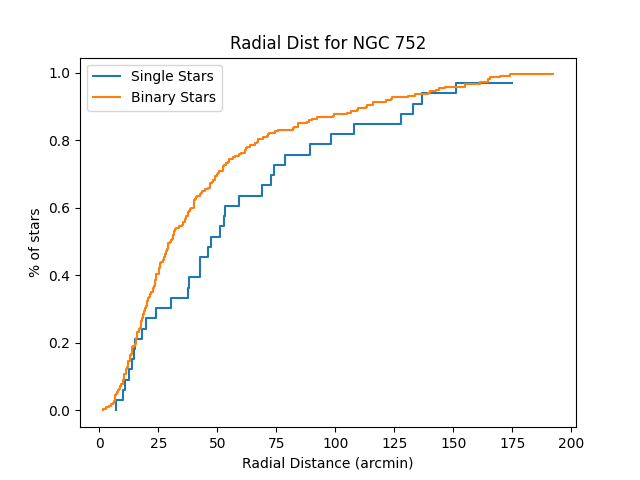
\includegraphics[width=\textwidth]{NGC 752_rad.png}
  \caption{NGC 752}
  \label{fig:im4}
 \end{subfigure}
~
\begin{subfigure}[b]{0.45\textwidth}
  \centering
  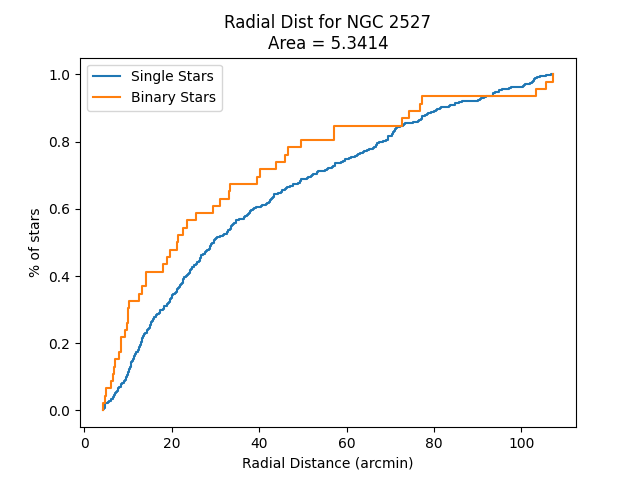
\includegraphics[width=\textwidth]{NGC 2527_rad.png}
  \caption{NGC 2527}
  \label{fig:im5}
\end{subfigure}
\caption{Radial Distribution for Star Clusters}
\label{fig:sim1}
\end{figure}

\section{King's Profile}
The King's profile\citep{kingprofile} is fitted for all the clusters in the study. The stars are divided into bins based on the radial distance from the cluster center. These bins are all annular rings of equal areas. This would mean the $n^{th}$ bin would be sandwiched between rings of radius $\sqrt{n-1}R$ and $\sqrt{n}R$ where $R$ is the radius of the cluster. After finding the number of stars in one bin, dividing that number by the area of the ring gives the surface density. When plotted against the radius on a log-log plot, we get a distribution of stars based on their proximities to the cluster center. Now we fit the curve given by the following equation to the data.
$$f = k \left( \frac{r_c}{\sqrt{r^2+r_c^2}} - \frac{r_t}{\sqrt{r_c^2+r_t^2}} \right) ^2$$
$k$ is an amplitude or a scaling factor, $r_c$ is the core radius and $r_t$ is the tidal radius. $k$ is simply the surface density of the innermost bin. $r_c$ and $r_t$ are the variable parameters which can be modified to get the best fit to the data. From the fitting procedure we can determine the core radius and tidal radius of the star cluster. The profile can be plotted easily with the \lstinline{astropy}\citep{astropy} module.



